\documentclass[12pt]{article}

% Layout.
\usepackage[top=1in, bottom=0.75in, left=1in, right=1in, headheight=1in, headsep=6pt]{geometry}

% Fonts.
\usepackage{mathptmx}
\usepackage[scaled=0.86]{helvet}
\renewcommand{\emph}[1]{\textsf{\textbf{#1}}}

% TiKZ.
\usepackage{tikz, pgfplots}

\usetikzlibrary{calc,trees,positioning,arrows,fit,shapes,through, backgrounds}
\usetikzlibrary{patterns}

\usetikzlibrary{decorations.markings}
\usetikzlibrary{arrows}

\usepackage{pgfplots}


% Misc packages.
\usepackage{amsmath,amssymb,latexsym}
\usepackage{graphicx}
\usepackage{array}
\usepackage{xcolor}
\usepackage{multicol}
\usepackage{fancyhdr}
\pagestyle{fancy}


% Misc.
\renewcommand{\d}{\displaystyle}
\newcommand{\ds}{\displaystyle}
\newcommand{\ul}[1]{\underline{#1}}
\def\bc{\begin{center}}
\def\ec{\end{center}}
\def\be{\begin{enumerate}}
\def\ee{\end{enumerate}}

\newcommand{\ans}[1][1in]{\rule{#1}{.5pt}}


\lhead{Math F113X: Quiz 5}
\rhead{March 7, 2025}

\begin{document}

\vspace{1cm}
\strut

\noindent \textbf{Name:} \hrulefill \quad  score:\ans[1cm] \ / 10 \\


\noindent There are 10 points possible on this quiz. No aids (book, notes, etc.)
are permitted. You may use a calculator.  {\bf Show all work and supporting calculations for full credit. Explain how you get your answers.}



\be

\item (3 points) Use Kruskal's Algorithm to find a minimum weight spanning tree in the graph below. A brief outline of Kruskal's Algorithm and a chart of edges ordered by weight is included.\\

\textbf{Kruskal's Algorithm:} Select the cheapest edge in the graph that does not create a circuit. Stop when a spanning tree is obtained.\\

\begin{minipage}{0.4\textwidth}
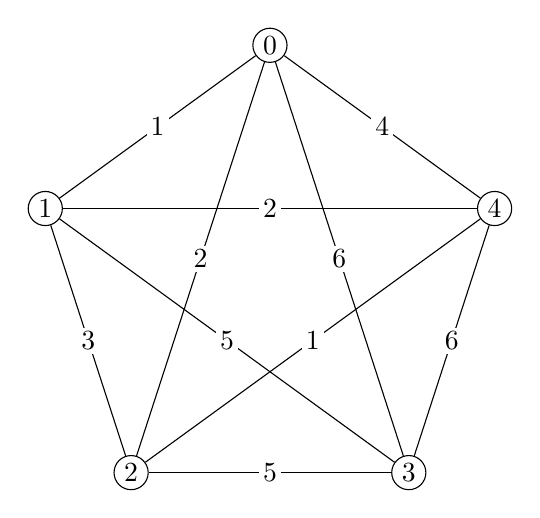
\begin{tikzpicture}[vtx/.style={draw, circle, inner sep =1.5 pt}, lbl/.style =  {inner sep =1.5 pt, fill = white}]
\foreach \i in {0,1,2,3,4}{\node[vtx] (\i) at (360*\i/5+90:3){\i};}
\foreach \i in {0,1,2,4}{\draw let \n1 = {int(mod(\i+1, 5))}, \n2 = {int(1*\i+1*\n1)}
 in (\i) -- node[lbl] {\n2} 
(\n1);}
\foreach \i in {0,1,2,4}{\draw let \n1 = {int(mod(\i+2, 5))}, \n2 = {int(mod(2*\i+1*\n1,7))}
in (\i) -- node[lbl] {\n2} 
(\n1);}
\draw (3) -- node[lbl] {6} (0);
\draw (3) -- node[lbl] {6} (4);
\end{tikzpicture}
\end{minipage}
\begin{tabular}{cc}
edge&weight\\
\hline \hline \\
01&1\\
24&1\\
02&2\\
14&2\\
12&3\\
04&4\\
13&5\\
23&5\\
03&6\\
34&6
\end{tabular}

\vfill

Draw the minimum weight spanning tree below: 

\begin{minipage}{0.4\textwidth}
\begin{tikzpicture}[vtx/.style={draw, circle, inner sep =1.5 pt}, lbl/.style =  {inner sep =1.5 pt, fill = white}]
\foreach \i in {0,1,2,3,4}{\node[vtx] (\i) at (360*\i/5+90:3){\i};}
\end{tikzpicture}
\end{minipage}
Minimum weight: \ans[2cm]
\vfill

\newpage
\item (3 points) Does the graph below contain an Euler circuit? An Euler path? You are \emph{not} asked to find one, only to determine if one exists. \emph{Justify your conclusion.}\\

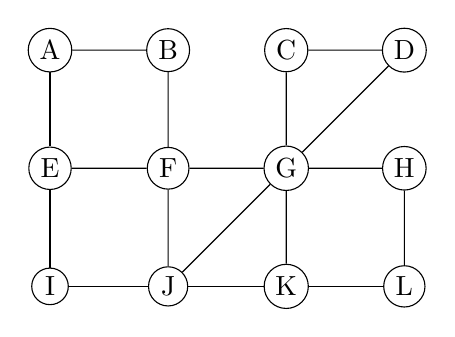
\begin{tikzpicture}[baseline=(current bounding box.center),scale=1.5]
\tikzstyle{vertex}=[circle, draw, inner sep=2pt]

\tikzstyle{every node} = [vertex];
\node (A) at (0,2) {A};
\node (B) at (1,2) {B};
\node (C) at (2,2) {C};
\node (D) at (3,2) {D};;
\node (E) at (0,1) {E};
\node (F) at (1,1){F};
\node (G) at (2,1){G};
\node (H) at (3,1){H};
\node (I) at (0,0) {I};
\node (J) at (1,0) {J};
\node (K) at (2,0) {K};
\node (L) at (3,0) {L};
\foreach \i/\j in {A/B,C/D,E/F,F/G,G/H,I/J,J/K,K/L,A/E,B/F,G/C,D/G,E/I,F/J,G/J,G/K,H/L}{\draw (\i) -- (\j);}
\end{tikzpicture}
\vfill


\item (4 points) Eulerize the graph below using as few edge duplications as possible. Then find an Euler circuit. Draw the circuit on the graph and list the vertices of your circuit in the space below.\\


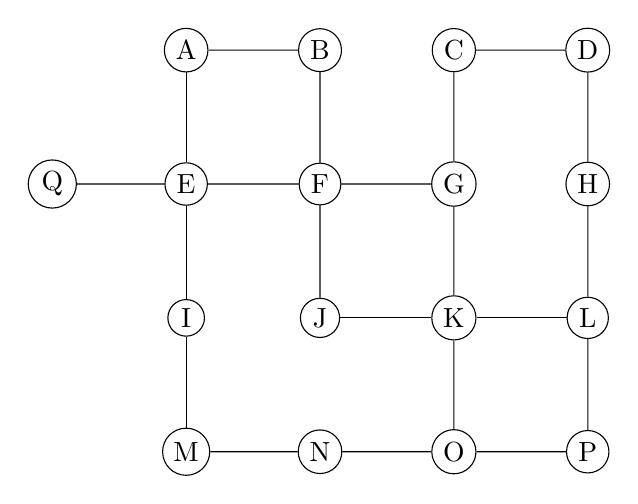
\begin{tikzpicture}[baseline=(current bounding box.center),lbl/.style={inner sep = 2pt, fill = white}, scale = 1.7]
\tikzstyle{vertex}=[circle, draw, inner sep=2pt]
\tikzstyle{every node} = [vertex];
\node (a) at (0,2) {A};
\node (b) at (1,2) {B};
\node (c) at (2,2) {C};
\node (d) at (3,2) {D};
\node (e) at (0,1) {E};
\node (f) at (1,1){F};
\node (g) at (2,1){G};
\node (h) at (3,1){H};
\node (i) at (0,0) {I};
\node (j) at (1,0) {J};
\node (k) at (2,0) {K};
\node (l) at (3,0) {L};
\node (m) at (0,-1) {M};
\node (n) at (1,-1) {N};
\node (o) at (2,-1) {O};
\node (p) at (3,-1) {P};
\node (q) at (-1,1) {Q};
\foreach \i/\j in {q/e,a/b,c/d,e/f,f/g,g/k,j/k,k/l,m/n,n/o,o/p,a/e,b/f,c/g,d/h,e/i,i/m,f/j,h/l,l/p,k/o}{\draw (\i) -- (\j);}
\end{tikzpicture}

\vfill
Euler circuit: \underline{\hspace{3in}}
 \ee
\end{document}